\chapter{Mission heritage} %Last updated 31-1-2016
\label{ch:missher}
In early 2012 a group of scientists and engineers was set-up to devise an approach for the continuing exploration of Mars \cite{mppg2012}. They had to combine all the requirements set by President Obama (to have humans in Mars orbit in the 2030s) and the 2011 NRC Decadal Survey for Planetary Science (science goals), while still keeping to the new proposed budget of the FY2013 U.S. Budget Submittal. Their conclusion was that a sample return mission would be the next logical step, because they deemed it to be the best compromise between human exploration, science and technology. They also suggested different mission architectures to perform an \ac{MSR} mission; using three, two or one launch(es). The first concept would first launch a rover to collect samples, then an \ac{MAV} and a so-called \textit{Fetch} rover to collect the sample case from the first rover and launch them into orbit, and the final launch would then sent a sample return orbiter to collect the \ac{MAV}/sample case and safely return it to Earth. The second concept would combine the last two launches into one using a smaller return orbiter propelled by a solar electric propulsion system. Finally, the third concept was to put all of these aspects into one launch, resulting in a sample collection rover with an on-board \ac{MAV} system and again a small return orbiter \cite{mppg2012}. Currently, NASA has decided to use a separate collector, orbiter and \ac{MAV} system, which is what the research topic is based on. With the topic defined as in \Cref{ch:oversub}, it is required to determine what has already been done and what is currently being researched. This is called researching the mission heritage and is performed for every of the three phases involved: Mars atmospheric ascent (\Cref{sec:maratascref}), low-thrust orbital transfers (\Cref{sec:lowthortrref}) and rendezvous between an ascent vehicle and an orbiting vehicle above a planet (\Cref{sec:asvehordirenref}). Both these last two sections will focus on the Earth, the Moon and Mars and will not involve trajectories between different celestial bodies. Finally, the \ac{MAV} heritage is examined in \Cref{sec:mav_des}. To keep an overview, the reference missions and research will be discussed per phase and in the same order as mentioned. 

\section{Mars atmospheric ascent reference missions}
\label{sec:maratascref}
To date there have not been any launches from the Martian surface back into space. This does not mean that there exist no reference missions or any reference research. In principle every Earth launch can be compared to a launch from the Martian surface; there is a noticeable gravitational acceleration, rotational speed and atmosphere. However, the Martian atmosphere is very thin with respect to the Earth atmosphere. In that sense, the Moon might be a better reference body. In this section research on Mars ascent will be discussed first, followed by actual flown Lunar sample return missions. Also, some Lunar ascent/sample return research will be discussed similar to the Mars studies and research.
%
%Also, a quick overview of known planned sample return missions with a proposed launch date will be given. 

\subsection{Martian ascent reference research}
\label{subsec:mars_res}
Research has been performed on Martian ascent trajectories and is still being carried out, for instance, by the \ac{DLR}. A list of reference research is shown in \Cref{tab:marsascent_refres} followed by a short summary of each of the researched cases.

\begin{table}[!ht]
\begin{center}
\caption{Previous and current Mars ascent trajectory research.}
\label{tab:marsascent_refres}
\begin{tabular}{|p{3cm}|p{3cm}|p{3cm}|l|l|}
\hline 
\textbf{Author} 	& \textbf{Organisation} & \textbf{Country} & \textbf{Year} & \textbf{Simulator} \\ \hline \hline
Fanning and Pierson \cite{fanning1996model} & Iowa State University & United States & 1996 & Unknown\\ \hline
Desai et al. \cite{desai1998}& NASA Langley and \ac{JPL} & USA & 1998 & \acs{POST} \& \acs{OTIS} \\ \hline
Whitehead \cite{whitehead2004mars,whitehead2005} & Lawrence Livermore National Laboratory & USA & 2004 & Unknown\\ \hline
Di Sotto et al. \cite{di2007system} & DEIMOS Engenharia and \acs{ESA} & Portugal/Europe & 2007 & Unknown\\ \hline
Trinidad et al. \cite{trinidad2012} & Northrop Grumman and \ac{JPL} & USA & 2012 & MCAT \\ \hline
Dumont \cite{dumont2015design}& \ac{DLR} 		& Germany & 2015 (Ongoing) & \acs{TOSCA} \\ \hline

%& & & \\ \hline
\end{tabular}
\end{center}
\end{table}

%Fanning and Pierson \cite{fanning1996model}
%Fanning and Pierson (\citeyear{fanning1996model})
%\citeauthor{fanning1996model} (\citeyear{fanning1996model})

\begin{description}
\item[Fanning and Pierson \cite{fanning1996model}]During the optimisation different ascent profiles were tested to find the optimal ascent trajectory from the Martian surface to a circular orbit around Mars. Two different models were used to observe the differences between them in the case of an optimisation for largest \ac{MAV} payload mass using a two-stage vehicle and thus minimising the propellant mass required. For the first and second stage a liquid XLR-132 and a liquid R-40B engine were assumed respectively. The target parking orbit had a radius of 3862.92 km (where they assumed a Mars radius of 3389.92 km resulting in a 473 km altitude). The two different used models were a gravity-turn model and a pitch-rate model. Using a constant \ac{GLOM} of 1400 kg, the gravity-turn model resulted in a maximum payload mass of 367.8 kg whereas the pitch-rate model resulted in 366.4 kg (or 366.8 kg when a higher pitch-rate was used). It was mentioned that the pitch-rate model might yield a better result overall if the aerodynamic effects are also taken into account but in the end it was concluded that the gravity-turn model is a good choice to reach a preliminary design for the \ac{MAV}.
\item[Desai et al. \cite{desai1998}] In this paper an \ac{MAV} ascent to a 300 km altitude circular orbit was simulated. The aerodynamic effects were simulated in a program called the Aerodynamic Preliminary Analysis System (APAS), which provides quick estimates of the aerodynamic parameters for different configurations. APAS thus allows for rapid phase 0 conceptual studies of different vehicle designs. The aero-thermodynamic properties were simulated in the Langley Aerothermodynamics Upwind Relaxation Algorithm (LAURA), which is a computational fluid dynamics code that provides solutions to the thin-layer Navier-Stokes equations. Finally, two different trajectory optimisation programs were used: the Program to Optimize Simulated Trajectories (POST) and the Optimal Trajectories by Implicit Simulation (OTIS) program. In POST, numerical integration is used to find the optimum trajectory and in OTIS uses a collocation scheme to perform the optimisation. Mars-\ac{GRAM} was used for the atmospheric model and the simulations also included mass, gravitational and propulsion models. Furthermore, a two-stage liquid propulsion system was assumed, which had to deliver a payload mass of 30 kg into space. It was concluded that aero-thermodynamic effects were minimal and the final nominal \ac{MAV} lift-off mass was found to be 426 kg. Unfortunately, all the software programs mentioned in this paper fall under the \ac{ITAR} of the United States \footnote{Personal correspondence with \ac{JPL} personnel} and can thus not be used by any foreign nationals.
\item[Whitehead \cite{whitehead2004mars,whitehead2005}] In both papers the circular target orbit was taken at an altitude of 500 km. Also it was assumed to have a 100 kg \ac{MAV} launch mass. Different trade-offs between staging, thrust, shape, and either liquid or solid propulsion were performed. In this case liquid propulsion showed a better performance with respect to the solid propulsion option. The problem was simulated as a simplified 2-D problem and coded into Fortran. It is also mentioned that miniaturisation of both liquid and solid propulsion systems would be required (down to a complete 10 kg system). A liquid single-stage to orbit is provided as a viable alternative.    
\item[Di Sotto et al. \cite{di2007system}]This research was performed as part of the European Aurora program (human space exploration program). The possible advantages of ascending to a 300 by 2000 km altitude parking orbit are discussed with respect to an ordinary 500 km altitude circular parking orbit. The optimisation of the trajectory was split into an atmospheric part and a so-called exo-atmospheric part. The first part was then again split into a vertical rise phase, constant pitch rate phase, constant pitch phase and gravity-turn phase respectively following \ac{MAV} launch. The second part was also split into several phases: first an active propulsion phase, then a coast phase, followed by another active propulsion phase where the steering resulted from using an optimum guidance law derived from the Primer vector method. In this case it was assumed that both the first (four engines) and second stage (one engine) used liquid Rocketdyne RS-2101c engines. It was concluded that a 300 by 2000 km altitude orbit could be achieved using the same architecture as for the 500 km altitude circular orbit. This would then also save 1000 kg in orbiter mass because of the higher altitude rendezvous.
% The used program optimised over 14 different optimisation variables and a number of constraints, where it was mentioned that the final orbital condition, the maximum propellant consumption, the maximum dynamic pressure peak and the aerothermal flux at fairing jettisoning were the most important constraints.
\item[Trinidad et al. \cite{trinidad2012}] In this paper the baseline design for the \ac{MAV} is discussed. Several trade-off's were made concerning the kind of propulsion system and propellants. Also, five different launch flight-path angles (aligned on the same longitude) were simulated and compared. This trajectory analysis was performed using a three degrees of freedom tool developed by Northrop Grumman called the Mission Capabilities Analysis Tool (MCAT). It used the Mars Geodetics and the 2010 atmosphere version of Mars-\ac{GRAM}. The program was used to optimise (through the change of steepness of the trajectory and relative size of each stage) for a minimum \ac{MAV} \ac{GLOM}. The trajectory analysis was performed at an orbit of 466 km above the Martian surface. The resulting lowest \ac{GLOM} was achieved using two liquid stages resulting in an \ac{MAV} mass of 227 kg (283 to 391 kg including contingencies). 
\item[Dumont \cite{dumont2015design}]\footnote{Information based on personal communications with author as well} \ac{TOSCA} is a program that has been under development by \ac{DLR}. It was initially created as an Earth launcher ascent simulator for early launcher design. Recently Dumont has started updating the program for both Lunar and Martian ascent, unfortunately nothing has been published yet on Martian ascent simulations. It incorporates both aerodynamic changes and propellant changes into the trajectory simulation and can also be used to optimise the trajectory based on several optimisation parameters. 
\end{description}
%
%Some of these simulation programs require an aerodynamic tool to simulate the aerodynamics of the \ac{MAV}, an aero-thermodynamic tool to simulate the thermal properties and the different models: atmospheric, gravitational, mass and propulsion characteristic models \cite{desai1998}. However, less complex simulation programs also provided an accurate initial impression of the trajectories.

%there were also more simplified simulation programs used which give a good initial impression of the trajectories.

\subsection{Reference flown Lunar sample return missions}
\label{subsec:lunarsrm}
As mentioned before, Lunar sample return missions can be considered similar to Mars sample return missions, one of the main difference being the atmosphere. This means that Lunar flight data can be used to validate the initial ascent program by assuming a Lunar ascent (and then changing the parameters to Martian parameters and adding the atmosphere in a later phase). A comprehensive overview of all the sample return missions is presented in \Cref{tab:prevmis} for both manned and unmanned missions \footnote{Overview: \url{https://en.wikipedia.org/wiki/Sample_return_mission} [Accessed 28 October 2015]}. All successful soil and rock sample return missions were performed by the Soviet Union (robotic) and the United States (manned). 

\begin{table}[!ht]
\begin{center}
\caption{Previous Lunar Sample Return Missions.}
\label{tab:prevmis}
\begin{tabular}{|l|l|l|c|}
\hline 
\textbf{Launch date} 		& \textbf{Country} & \textbf{Mission} & \textbf{Returned mass [kg]} \\ \hline \hline
16 July 1969 		& USA & Apollo 11 & 22  \\ \hline
14 November 1969 		& USA & Apollo 12 & 34  \\ \hline
12 September 1970 		& Soviet Union & Luna 16 & 0.101  \\ \hline
31 January 1971 		& USA & Apollo 14 & 43  \\ \hline
26 July 1971 		& USA & Apollo 15 & 77 \\ \hline
14 February 1972 		& Soviet Union & Luna 20 & 0.055  \\ \hline
16 April 1972 		& USA & Apollo 16 & 95  \\ \hline
7 December 1972 		& USA & Apollo 17 & 111  \\ \hline
9 August 1976 		& Soviet Union & Luna 24 & 0.17  \\ \hline
\end{tabular}
\end{center}
\end{table}

Both Luna and Apollo missions first landed a craft on the Moon, then collected samples and returned these samples using a Lunar ascent vehicle. Some data on the Luna missions is provided in \cite{harvey2007soviet}. Unfortunately, it does not provide enough information on the ascent trajectory of the Luna return vehicles and therefore the Luna missions cannot be used for validation. The Apollo missions were, however, documented in detail and do include ascent flight data \cite{apollo1971}.\\
%The Apollo programme was the first and only manned Lunar programme. It started in 1961 and lasted till 1972 \cite{wiki_apollo}. The first missions were designed as tests and demonstrators for the actual Lunar landings. The first manned Lunar landing was performed by the Apollo 11 crew on 20 July 1969 \cite{apollo1971}. Another five successful manned Lunar missions followed: Apollo 12, 14, 15, 16 and 17. All Apollo missions were able to bring back tens of kilograms of soil and rock samples. Both the astronauts and the samples ascended from the Lunar surface using the \ac{LAM}. Once back in Lunar orbit, the \ac{LAM} would rendezvous with the \ac{CSM} at which time the astronauts and all the samples were transferred to the \ac{CSM}. The \ac{LAM} was discarded and the \ac{CSM} was used to return to Earth. Both \ac{LAM} and \ac{CSM} are depicted in \Cref{fig:lam_and_cm_wiki_lm}.
%
%
%\begin{figure}[!ht]
%\centering
%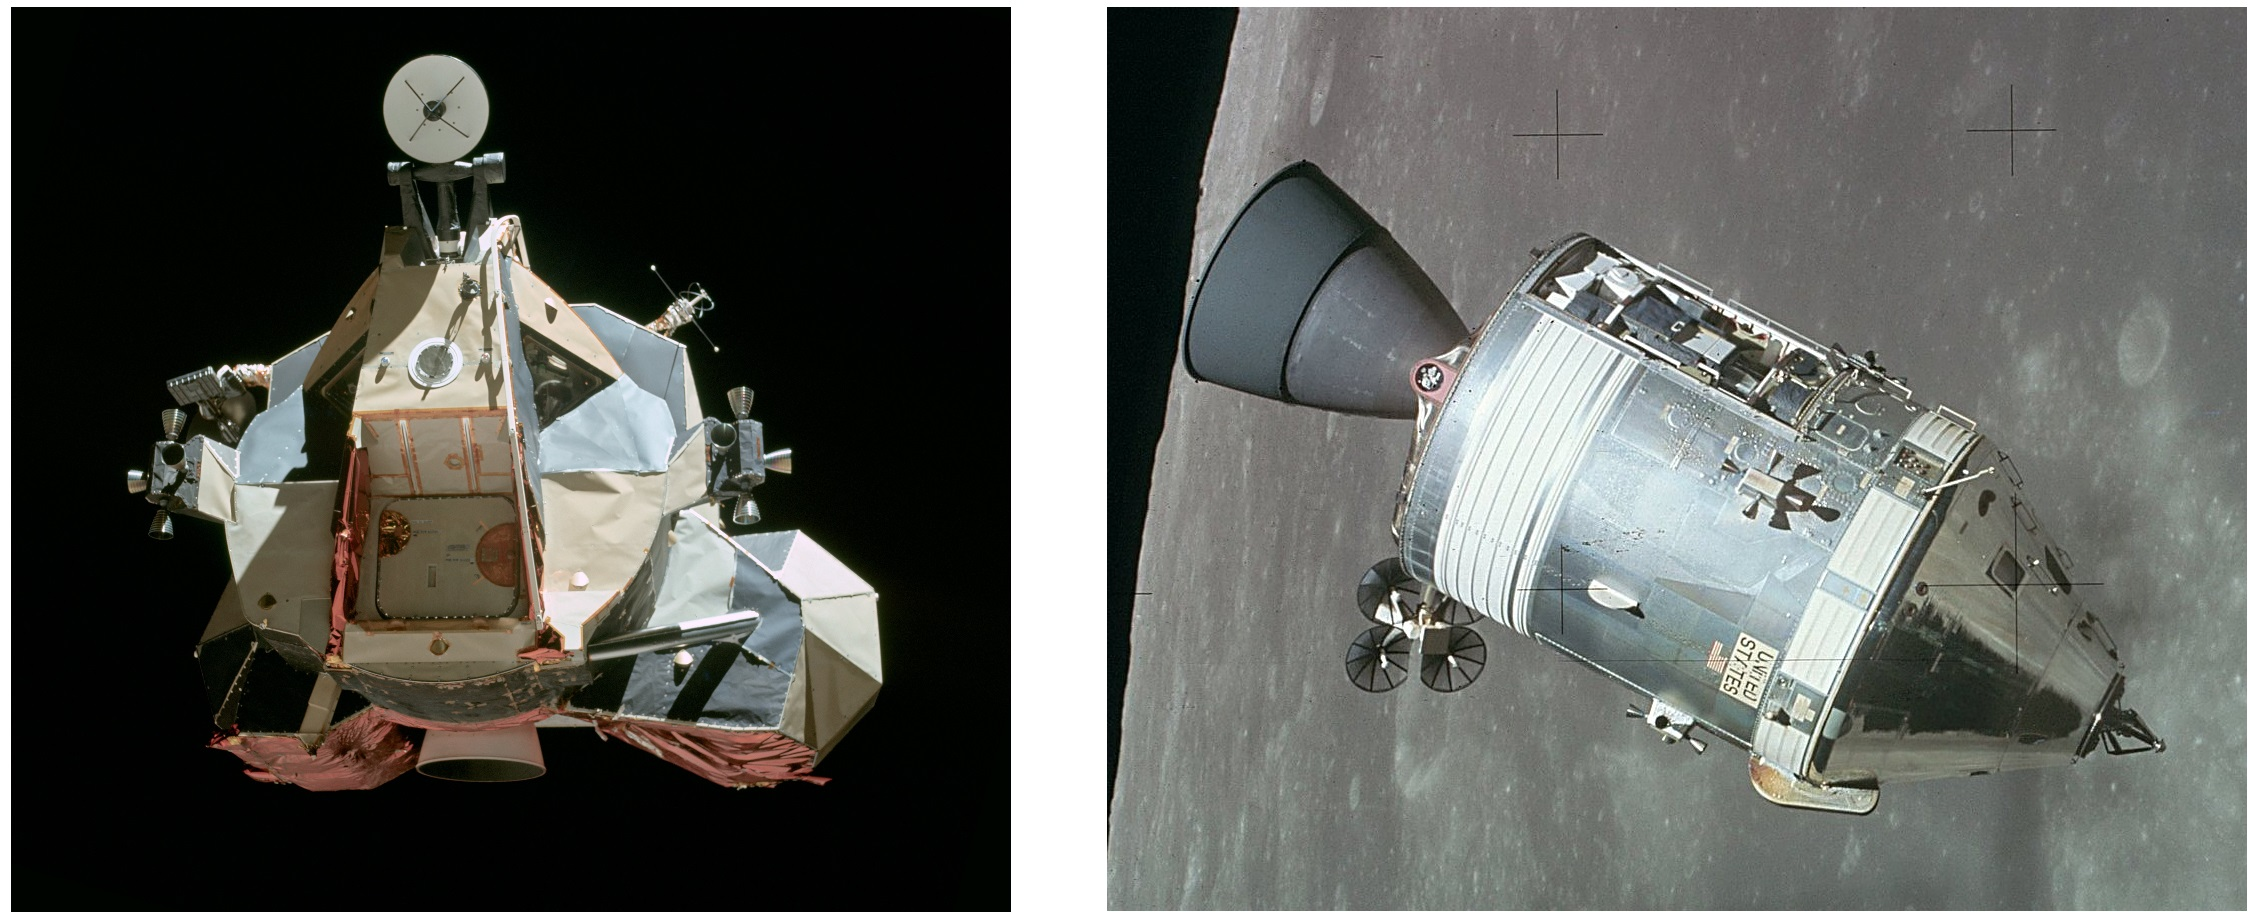
\includegraphics[width=0.5\textwidth]{figures/heritage/lam_and_cm_wiki_lm.jpg}
%\caption{Left: Lunar Ascent Module, Right: Apollo Command and Service Module. Source: NASA}
%\label{fig:lam_and_cm_wiki_lm}
%\end{figure}


%, which was the upper part of the \ac{LM} as shown in \Cref{fig:lm_wiki_apollo,fig:lam_wiki_lm}.



%\begin{figure}[!ht]
%\centering
%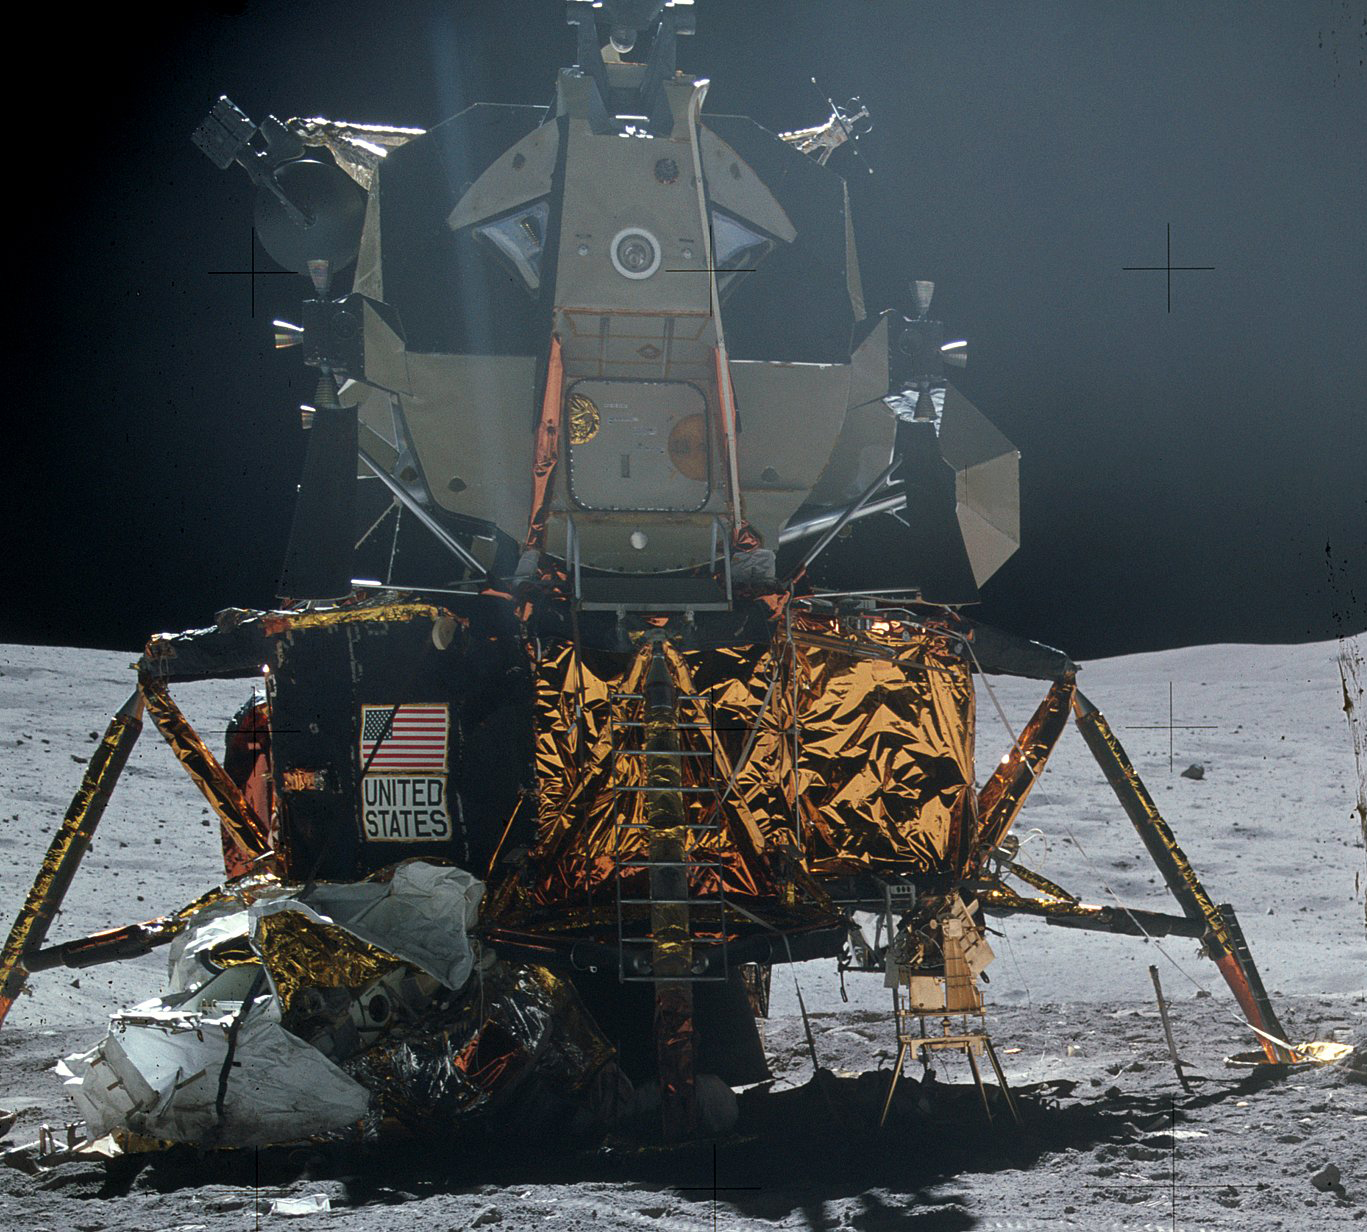
\includegraphics[width=0.5\textwidth]{figures/heritage/lm_wiki_apollo.jpg}
%\caption{Lunar Module \cite{wiki_apollo}}
%\label{fig:lm_wiki_apollo}
%\end{figure} 
%
%
%
%\begin{figure}[!ht]
%\centering
%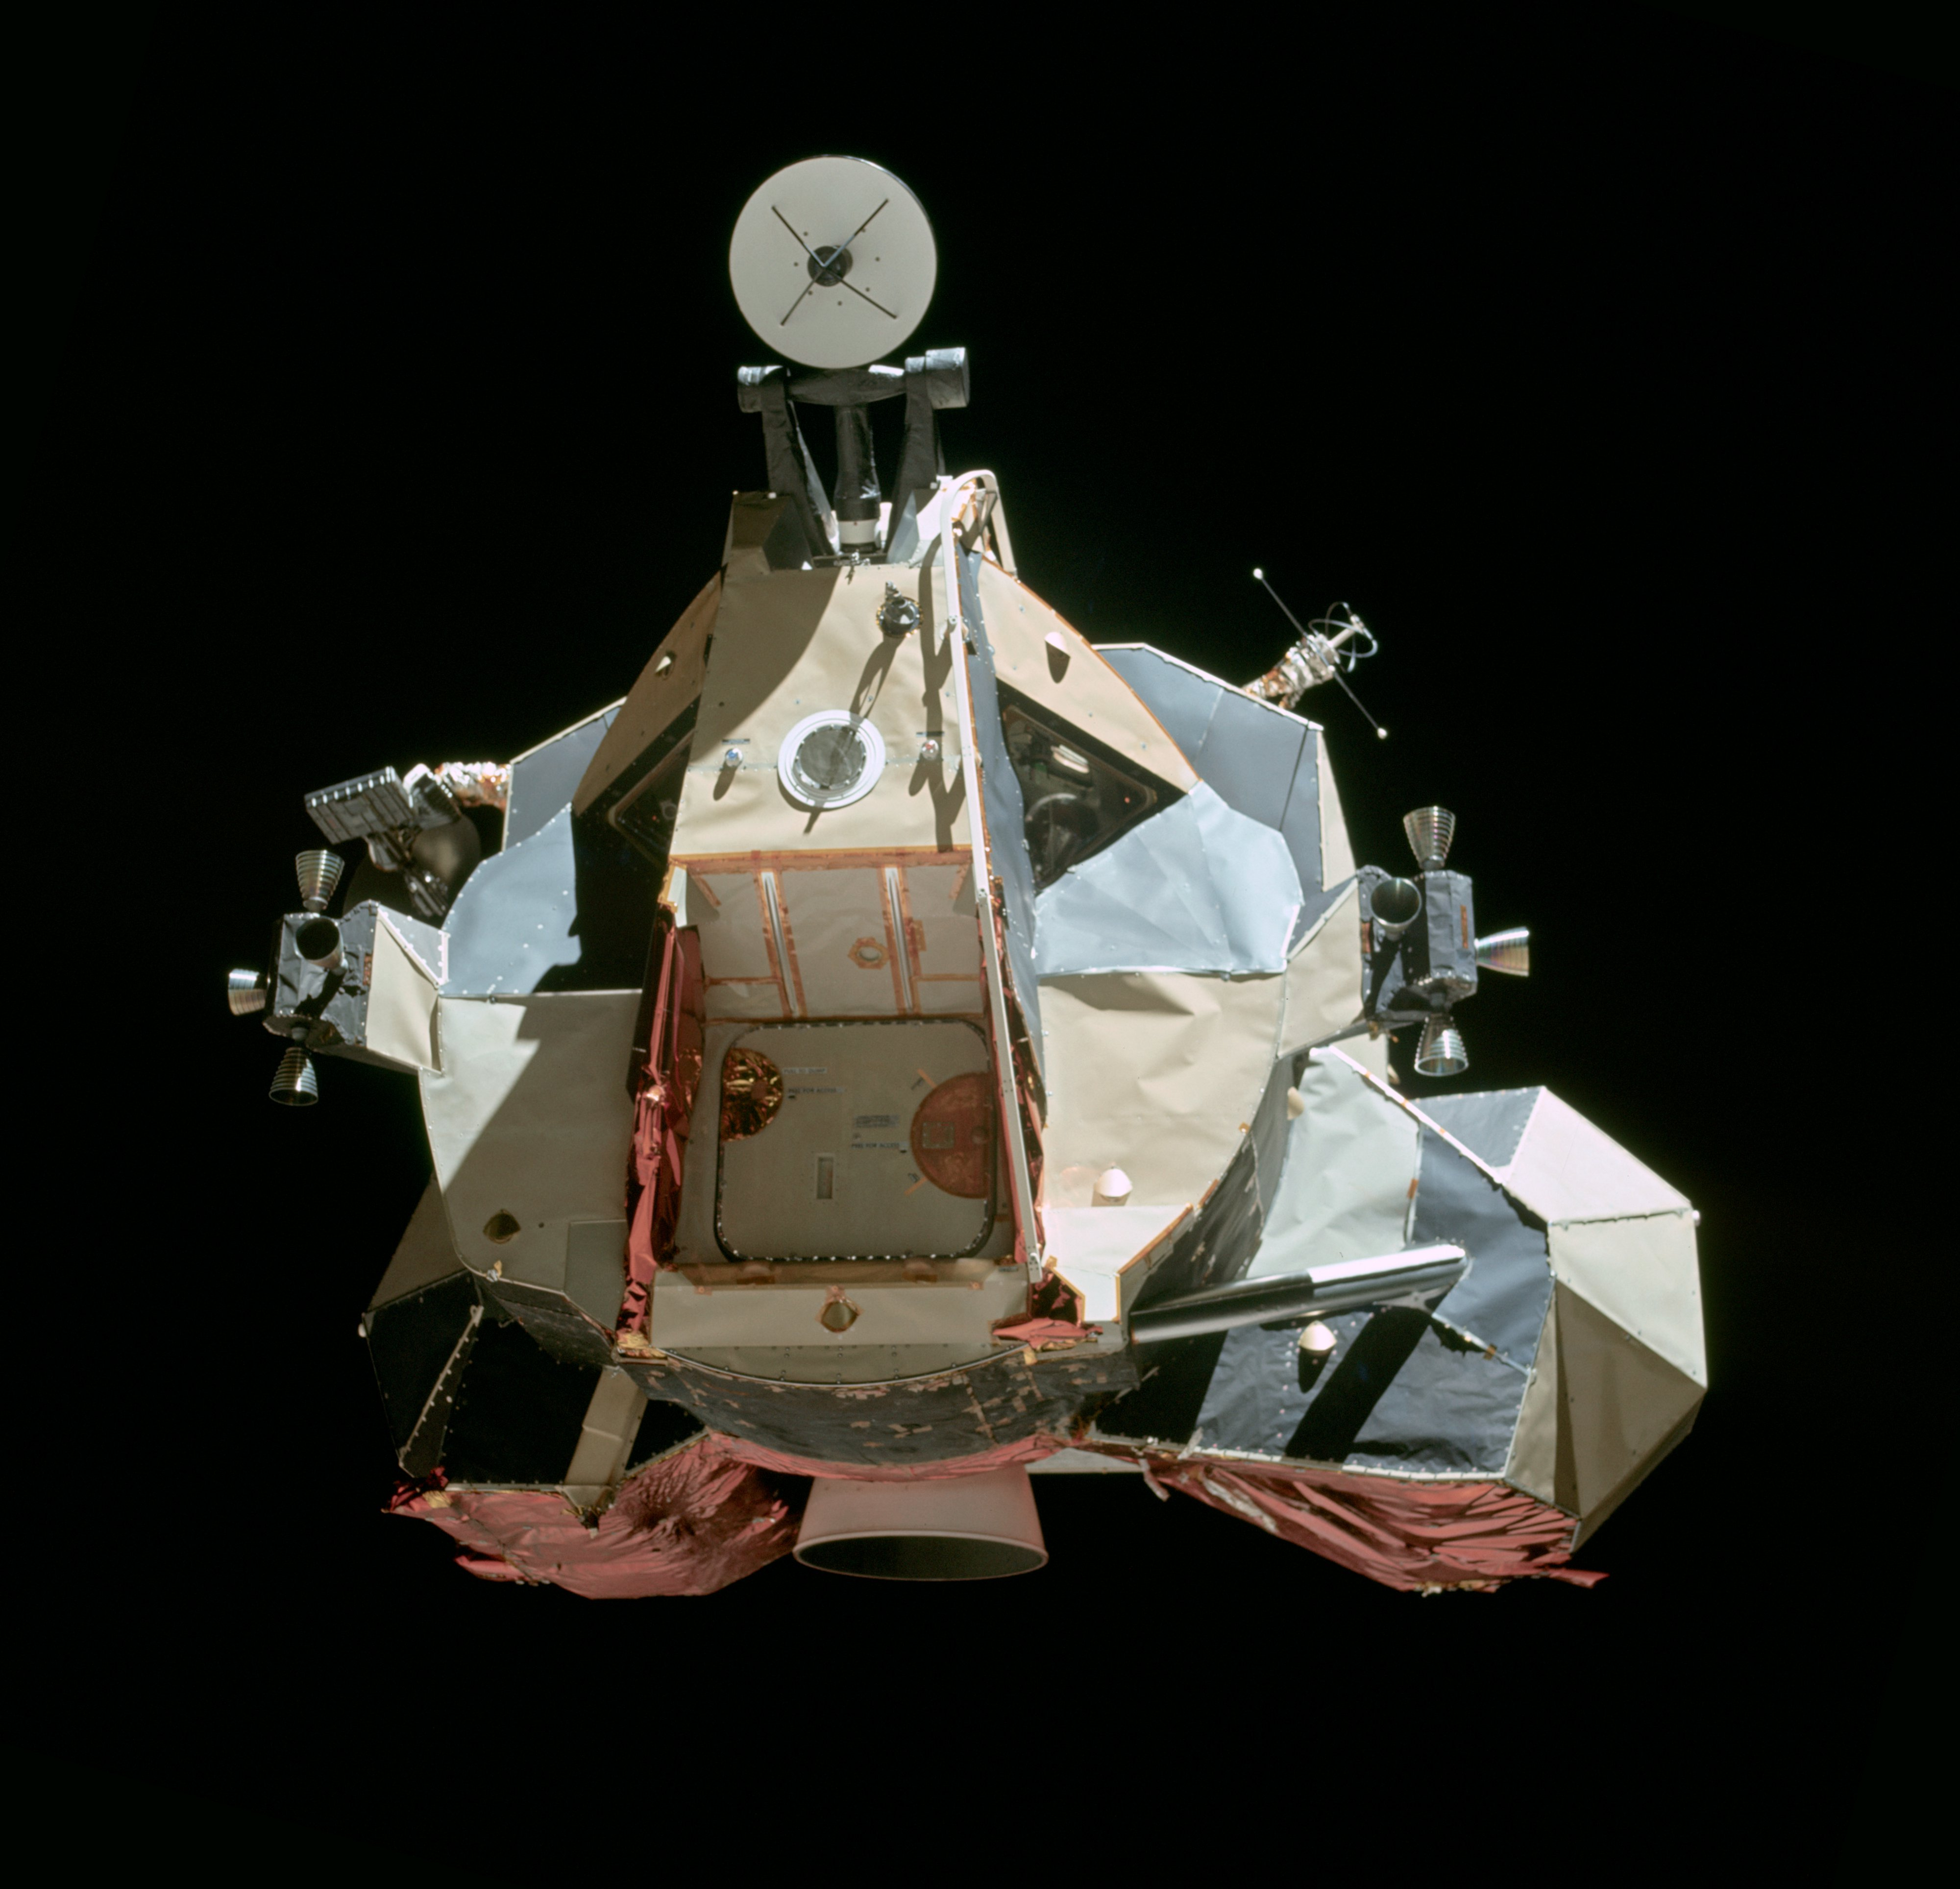
\includegraphics[width=0.5\textwidth]{figures/heritage/lam_wiki_lm.jpg}
%\caption{Lunar Ascent Module \cite{wiki_lm}}
%\label{fig:lam_wiki_lm}
%\end{figure}



%The \ac{CSM} incorporated an Earth return capsule (\ac{CM}) for Earth re-entry in the 'nose' of the vehicle, as can be identified in \Cref{fig:cm_wiki_cm}. The \ac{CM} would separate from the \ac{SM} just before entering the atmosphere. \Cref{fig:capsule_wiki_cm} shows a photo of the Apollo return capsule after re-entry.   

%\begin{figure}[!ht]
%\centering
%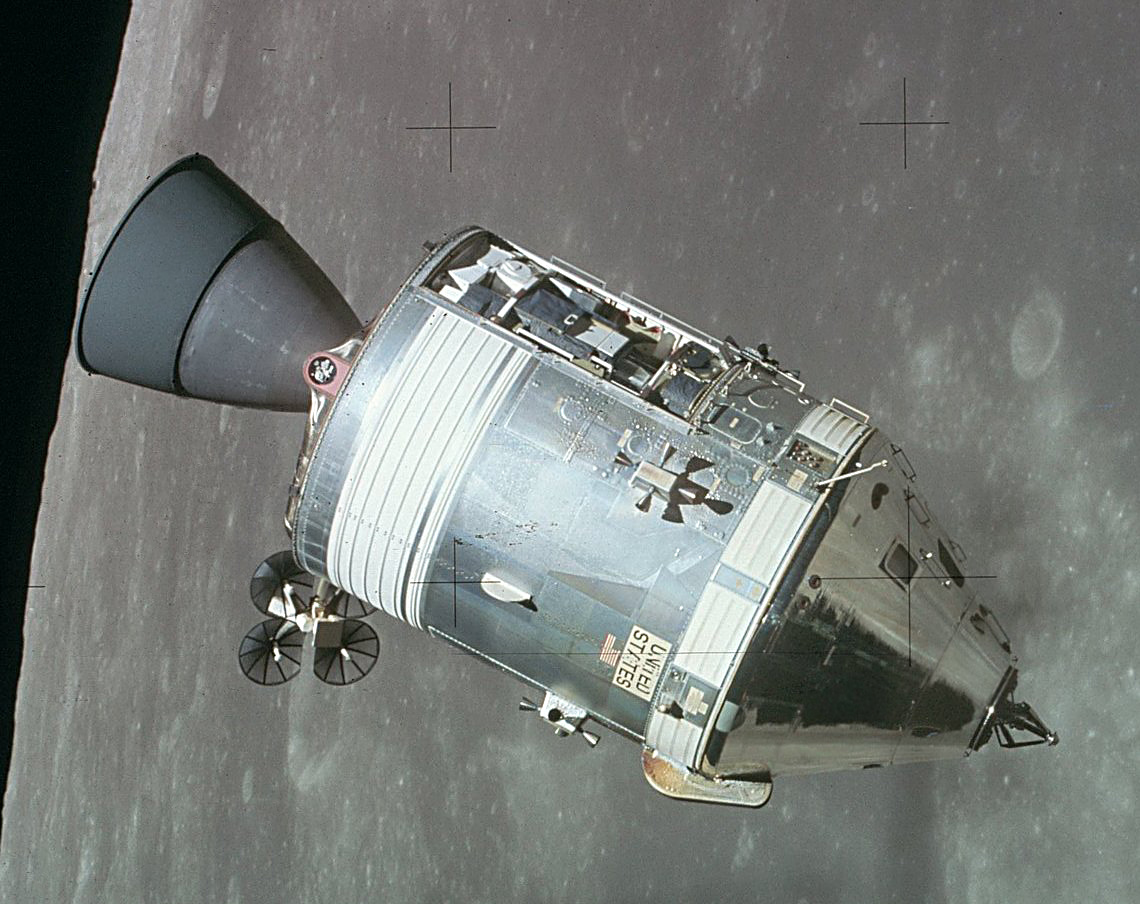
\includegraphics[width=0.5\textwidth]{figures/heritage/cm_wiki_cm.jpg}
%\caption{Apollo Command and Service Module \cite{wiki_cm}}
%\label{fig:cm_wiki_cm}
%\end{figure}
%
%\begin{figure}[!ht]
%\centering
%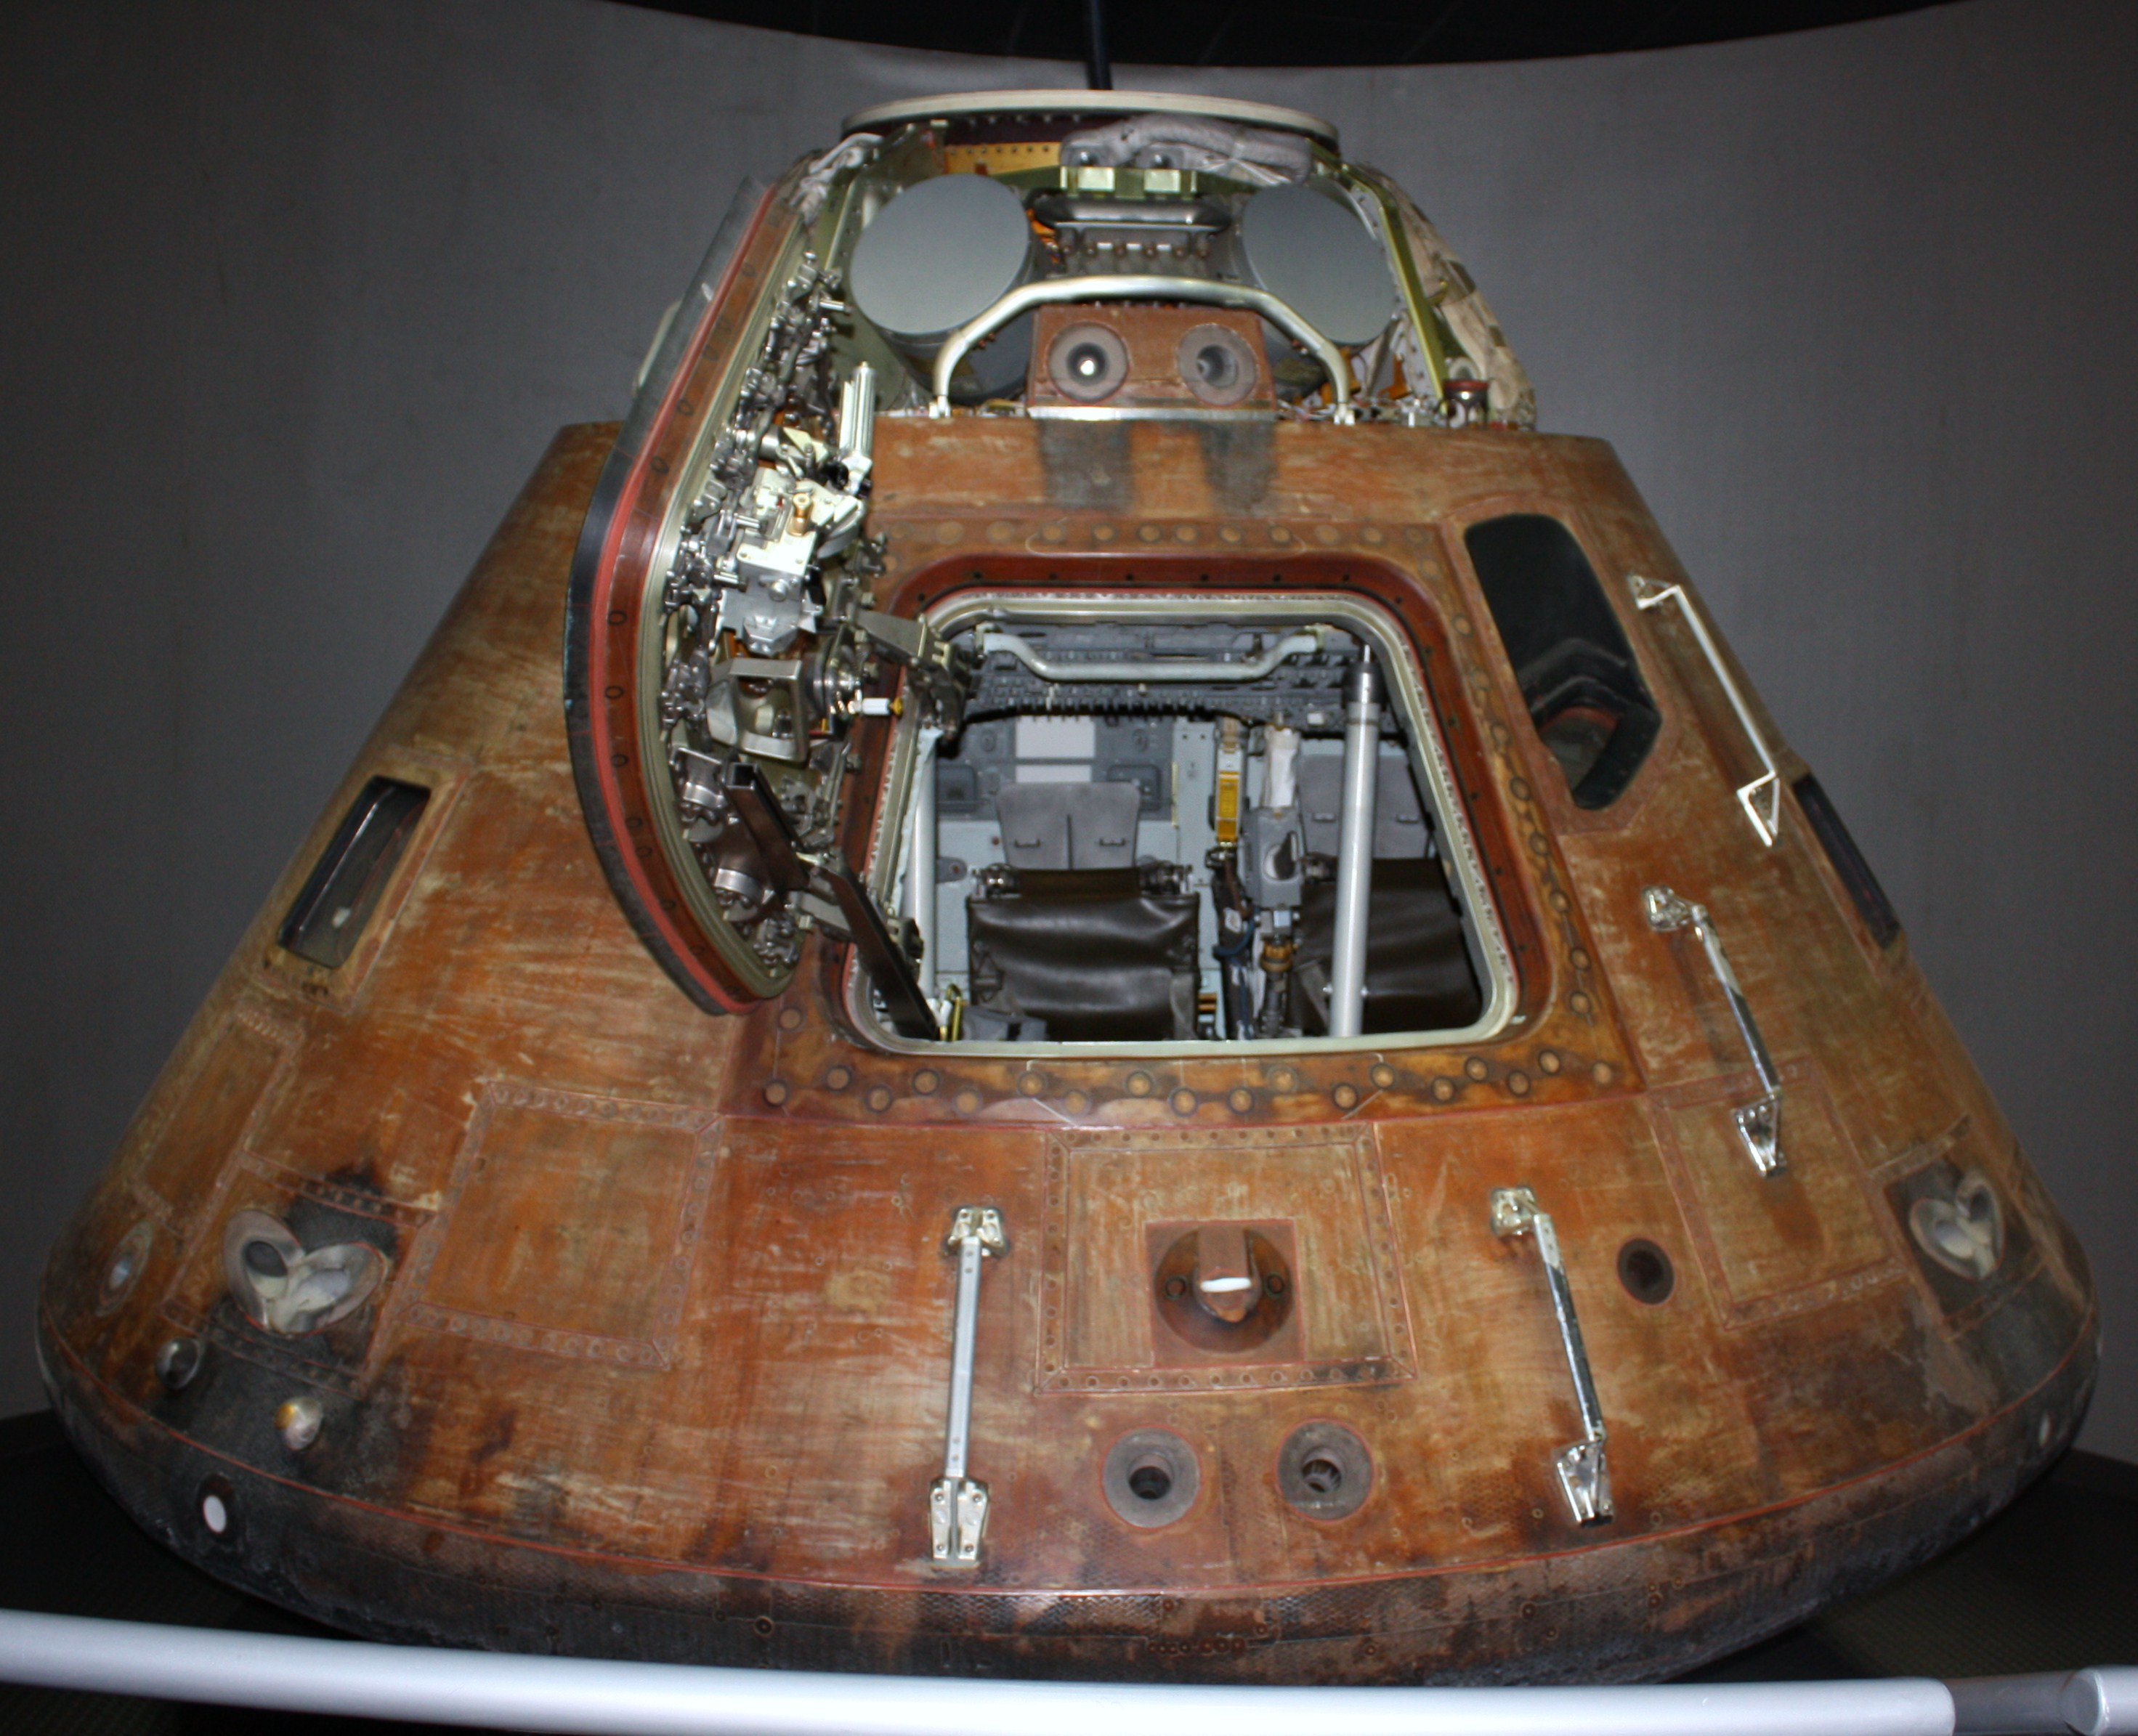
\includegraphics[width=0.5\textwidth]{figures/heritage/capsule_wiki_cm.jpg}
%\caption{Apollo re-entry capsule \cite{wiki_cm}}
%\label{fig:capsule_wiki_cm}
%\end{figure}

%The details of the Apollo (and the other) missions will be discussed in the corresponding subject chapters later in this report.

%\paragraph{Luna}
%The Luna programme was a Soviet Lunar exploration programme between 1958 and 1976 \cite{christy2015}. It was first proposed by Sergei Korolev on the 28th of January 1958. The programme started with some early probing between 1958 and 1960 by the Luna 1, 2 and 3 probes, followed by a proof of technology by the Luna 4 through 14 missions between 1963 and 1968. On the 3rd of February 1966, Luna 9 performed the first successful soft Lunar landing. Following this successful mission, 6 more Lunar landing missions were completed successfully: Luna 13, 16, 17, 20, 21 and 24. Luna 23 did land on the moon, but was not able to perform its mission after that because of damage which occurred during this landing. \\
%As mentioned in \Cref{tab:prevmis} Luna 16, 20 and 24 were sample return missions (also see \cite{luna2015}).
%% 17 and 21 were rover missions 
%These three missions were virtually identical in their architecture and \ac{s/c} design. The \ac{s/c} consisted of a descent stage and a smaller ascent stage \cite{grayzeck2014}. General information on the \ac{s/c} itself can be found in \cite{luna16_esp}. The \ac{s/c} had a drill on board that was attached to an arm that could be rotated in one direction. Basically it could lower down to the surface to drill and collect the samples and then move up towards the ascent stage to deposit the samples. The ascent stage would then lift-off with the samples contained in a spherical re-entry capsule (also see \Cref{fig:luna16_sequence_capcom_fr}). This spherical capsule would then perform a ballistic re-entry and land in Soviet controlled territory. 
%
%
%\begin{figure}[!ht]
%\centering
%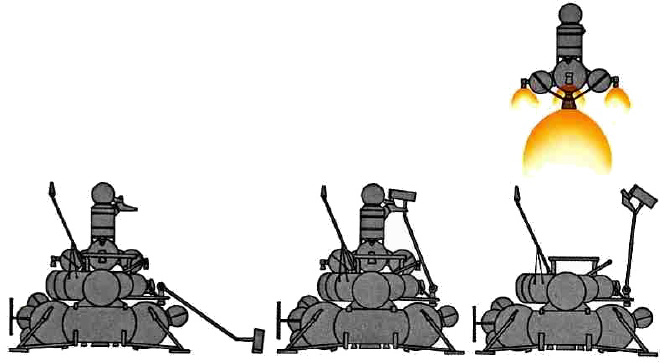
\includegraphics[width=0.7\textwidth]{figures/heritage/luna16_sequence_capcom_fr.jpg}
%\caption{Luna sample return sequence \cite{capcom_fr}}
%\label{fig:luna16_sequence_capcom_fr}
%\end{figure}




%\subsection{Planned Sample Return Missions}
%\label{subsec:planmis}
%Two of the planned missions to Mars were already discussed earlier, the Mars 2020 deploying a rover that will collect samples, and the \ac{MSR} mission to bring samples back to Earth. Both of these missions are under consideration by \ac{JPL}. However, besides these missions, there are other sample return missions planned by the United States and other countries. An overview of the other missions is given in \Cref{tab:planmis}. The last one mentioned is based on SpaceX technology and is not an official running programme at this time but could be interesting in the future. 
% 
%\begin{table}[!ht]
%\begin{center}
%\caption{Other planned sample return missions}
%\label{tab:planmis}
%\begin{tabular}{|l|l|l|l|p{3cm}|}
%\hline 
%\textbf{(Proposed) Launch date} 		& \textbf{Country} & \textbf{Mission} & \textbf{Target} & \textbf{Kind of mission} \\ \hline \hline
%3 December 2014 		& Japan & Hayabusa 2 & Asteroid 1999 JU3 & Surface samples \cite{hayabusa2_2014} \\ \hline		
%3 September 2016	& United States & OSIRIS-REx & Asteroid Bennu & Surface samples up to 2 $kg$ \cite{osiris2015} \\ \hline
%2017		& China & Chang'e 5 & Moon & At least 2 $kg$ of soil and rock samples \cite{wiki_change5} \\ \hline
%2022	& United States & Red Dragon & Mars & Soil and rock samples \cite{david2014} \\ \hline
%\end{tabular}
%\end{center}
%\end{table}
%
%Both the Hayabusa 2 and OSIRIS-REx missions will not actually land on their visiting bodies, so will not be used as reference when it comes to launching from the surface of a another celestial body.\\
%
%A different sample return mission competing with OSIRIS-REx to be selected was MoonRise. This completely robotic mission was planned to be launched in late 2016 and collect samples from the far-side of the moon \cite{alkalai2010moonrise}. The robotic mission would land at the South Pole-Aitken Basin and ascent back to Earth with samples collected. Unfortunately OSIRIS-REx was chosen instead \cite{brown2009nasa,jpl_missions}. 


   
% I deemed this paragraph useless for the current thesis topic (did not add anything)






\subsection{Lunar ascent reference research}
\label{subsec:lunar_res}
Research on Lunar sample return can also be used as reference data. Therefore a similar table to \Cref{tab:marsascent_refres} can be set-up for Lunar research. An overview of different Lunar ascent/sample return research is provided in \Cref{tab:moonascent_refres}. It is interesting to see that different studies use different Lunar ascent vehicle configurations and propulsion systems based on the requirements for each study case.

\begin{table}[!ht]
\begin{center}
\caption{Previous and current Lunar ascent trajectory research.}
\label{tab:moonascent_refres}
\begin{tabular}{|p{3cm}|p{3cm}|p{3cm}|l|l|}
\hline 
\textbf{Author} 	& \textbf{Organisation} & \textbf{Country} & \textbf{Year} & \textbf{Program name} \\ \hline \hline
Sostaric and Merriam \cite{sostaric2008lunar}& NASA Johnson Space Center & USA & 2008 (Ongoing) & SORT\\ \hline
Dietrich et al. \cite{dietrich2015ascent} & University of Colorado & USA & 2015 & Copernicus\\ \hline
Dumont \cite{dumont2015design} & \ac{DLR} 		& Germany & 2015 (Ongoing) & \acs{TOSCA} \\ \hline

%& & & & \\ \hline
\end{tabular}
\end{center}
\end{table}


\begin{description}
\item[Sostaric and Merriam \cite{sostaric2008lunar}]In this paper manned Lunar ascent and rendezvous trajectories were simulated and optimised. This was accomplished by dividing the ascent up into three different parts. A 100 m vertical rise, followed by a single-axis rotation manoeuvre and ending in a powered explicit guidance phase to reach the target orbit. The problem was simulated in a 3-degrees of freedom simulation program called SORT. The single-axis rotation algorithm calculates a time-optimal single-axis rotation given the initial and final attitude. For the final phase of the ascent an optimiser called NPSOL was used, which is a non-linear programming solver. The initial target orbit was 15.24 by 75 km above the Lunar surface. The possibilities for emergency ascent were investigated together with a comparison between yaw steering and on-orbit plane changes. It was concluded that for large plane changes it is best to perform the plane changes on-orbit to reduce the required $\Delta V$.
\item[Dietrich et al. \cite{dietrich2015ascent}]In 2013 a new research study was performed called Orion/MoonRise where the MoonRise mission would be combined with a manned mission to a halo orbit around the Earth-Moon L2 point \cite{alkalai2013orion}. In that case the MoonRise probe would be modified slightly and would have to ascent from the surface of the Moon to the Orion \ac{s/c} in its halo orbit. The simulations performed showed a maximum theoretical sample return mass of 38 kg. The ascent vehicle would use a single solid STAR 48AX motor, based on the STAR 48A and 48B motors, and would have to be specially designed by Orbital ATK. In this follow-up study two possible landing/ascent points on the Moon were investigated: Schr\"{o}dinger Crater and Tsiolkovsky Crater \cite{dietrich2015ascent}. The simulator was developed in a tool called Copernicus combined with a MATLAB interface. The trajectories were simulated to ascent from the Lunar surface to a halo orbit around L2 and were split into four parts: ascent, trajectory correction manoeuvre, halo orbit insertion and halo orbit propagation.
\item[Dumont \cite{dumont2015design}] Lunar ascent simulations were performed using \ac{TOSCA} in light of the ROBEX project. In this study, a re-usable concept Lunar ascent vehicle is described using a liquid oxygen/liquid hydrogen propulsion system with a specific impulse ($I_{sp}$) of 440 s. The target orbit was 15 by 100 km after which the orbit would be circularised to 100 km. Ascent altitude-time profiles are provided for two different constant thrust settings: 25.9 and 34.5 kN.
\end{description}

\nomenclature[R5]{$I_{sp}$}{Specific impulse\nomunit{s}}

%For the Lunar ascent simulation part of \ac{TOSCA} verification and validation has been started and performed in early 2015 and it is still being improved. A publication with applications for the ROBEX mission is currently under review and will hopefully be published within the next six months. \textbf{\textcolor{red}{Include newly received paper Etienne!}}


%\textbf{\textcolor{red}{Include more Lunar ascent research?}}






\section{Low-thrust orbital transfer reference missions}
\label{sec:lowthortrref}
Because the planned Mars 2022 orbiter, which will likely collect the Martian sample from the \ac{MAV} and return back to Earth, will have a low-thrust propulsion system it is important to identify previous missions and research. In the past few years, low-thrust propulsion systems have become increasingly popular in long-duration missions because of the high $I_{sp}$ and the low total system mass. Since the current defined topic will focus on a low-thrust problem in the Martian system, it is useful to analyse the propulsion system and the trajectories flown by previous low-thrust missions in planetary systems (see \Cref{subsec:earthlowthrust}). To date, no low-thrust missions have flown in the Martian system. However, research has been performed on low-thrust missions in both the Earth and Martian system as described in \Cref{subsec:lowrefres}.

%Also, to look at general low-thrust optimisation and propagation problems it is useful to look at interplanetary low-thrust missions as well.

\subsection{Earth system low-thrust applications}
\label{subsec:earthlowthrust}
Low-thrust applications in the Earth system were first implemented back in the 60s with the first (non-experimental) flight, using \ac{EP} for attitude control, performed by the Zond-2 \cite{martinez1998spacecraft}. The three main applications for \ac{EP} in satellites have historically been in attitude control, (geosynchronous) station keeping and other general orbit adjustments. For the thesis problem it is interesting to investigate missions that used \ac{EP} for orbit transfers and orbital phase changes. \Cref{tab:prevlowthrustmis} provides an overview of different missions that used electric propulsion \acsu{EP} as a means to perform either orbital phase adjustments or orbit transfers (based on \cite{martinez1998spacecraft}). In the past few years \ac{EP} has become increasingly popular for use as \ac{s/c} main propulsion systems and now companies, such as Boeing and their 702SP series of communication satellites\footnote{Boeing company: \url{http://www.boeing.com/resources/boeingdotcom/space/boeing_satellite_family/pdf/Bkgd_702SP.pdf} [Accessed 25 November 2015]}, are even introducing fully electric \ac{s/c} \cite{schaeff2014low}. These new satellites are also included in \Cref{tab:prevlowthrustmis} as well as a number of missions which had to use their \ac{EP} systems for orbital transfer manoeuvres even though the electric thrusters were not intended for it\footnote{Artemis mission update: \url{http://www.esa.int/Our_Activities/Telecommunications_Integrated_Applications/Artemis_finally_reaches_operational_orbit} [Accessed 18 October 2015]}$^{,}$\footnote{AEHF-1 mission update: \url{http://spaceflightnow.com/atlas/av019/111009.html} [Accessed 18 October 2015]}. 


\begin{table}[!ht]
\begin{center}
\caption{Previous Low-thrust Earth Missions.}
\label{tab:prevlowthrustmis}
\begin{tabular}{|l|l|l|c|}
\hline 
\textbf{Launch year} 		& \textbf{Country} & \textbf{Mission} & \textbf{\ac{EP} use} \\ \hline \hline
1965 & USA & Vela & Phase adjustment \\ \hline
1967 & USA & Advanced Vela & Phase adjustment \\ \hline
1988 & USA & Gstar-3 & Orbit Transfer \\ \hline
%1998 & USA & New Millenium, DS-1 & Orbit Transfer \\ \hline
2000 & USA & MightySat II.1 & Orbit Transfer \\ \hline
2001 & Europe & Artemis & Orbit Transfer \\ \hline
2010 & USA & AEHF(-1) & Orbit Transfer \\ \hline
2015 & USA & ABS-3A & Orbit Transfer \\ \hline
2015 & USA/France & Eutelsat 115 West B  & Orbit Transfer\\ \hline
 
\end{tabular}
\end{center}
\end{table}

Compared to the intended use of the low-thrust \ac{EP} on the Mars 2022 orbiter, where the propulsion system shall be used to perform several orbital transfer manoeuvres including orbit raising, orbit lowering and most likely inclination changes, the orbit transfer applications for the satellites shown in \Cref{tab:prevlowthrustmis} are simply transferring the \ac{s/c} from a \ac{LEO} or \ac{GTO} to \ac{GEO}. Advanced low-thrust manoeuvres have been performed by interplanetary missions, however non-planetary missions are not included in this report.





%\textbf{\textcolor{red}{Should I include this part?}} Nope..

\subsection{Low-thrust (Martian) planetary system reference research}
\label{subsec:lowrefres}
Because low-thrust as a main propulsion system has become increasingly important, many studies are currently being conducted in the area of low-thrust trajectory optimisation for the Earth system, Mars system and mainly interplanetary transfers. However, since this problem deals with the orbit transfers in a planetary system the reference research will be selected based on Earth and Martian system applications. The reference research is presented in \Cref{tab:marslow_refres} again followed by a short description.  


\begin{table}[!ht]
\begin{center}
\caption{Previous and current Mars low-thrust trajectory research.}
\label{tab:marslow_refres}
\begin{tabular}{|p{3cm}|p{3cm}|l|l|p{3cm}|}
\hline 
\textbf{Author} 	& \textbf{Organisation} & \textbf{Country} & \textbf{Year} & \textbf{Program name} \\ \hline \hline
Geffroy and Epenoy  \cite{geffroy1997optimal} & \acs{CNES} & France & 1997 & Unknown \\ \hline
Kluever and Oleson \cite{kluever1998direct} & University of Missouri-Columbia and NYMA, Inc. & USA & 1998 & Unknown \\ \hline
Bertrand et al. \cite{bertrand2001electric} & \acs{CNRS} \& \acs{CNES} & France & 2001 & Unknown\\ \hline
Whiffen \cite{whiffen2006mystic} & NASA \ac{JPL} & USA & 2006 & Mystic\\ \hline
Sims et al. \cite{sims2006implementation} & NASA \ac{JPL} & USA & 2006 & MALTO \\ \hline
Kos et al.  \cite{kos2006overview} & NASA \ac{JPL} & USA & 2006 & MALTO, Mystic, Copernicus, OTIS, SNAP, CHEBYTOP, VARITOP, SEPTOP, NEWSEP and Sail \\ \hline
Derz and Seboldt \cite{derz2012mars} & \ac{DLR} & Germany & 2012 & InTrance \\ \hline



%& & & & \\ \hline
\end{tabular}
\end{center}
\end{table}

\begin{description}
\item[Geffroy and Epenoy  \cite{geffroy1997optimal}] The possibility of using a generalised version of averaging techniques for low-thrust optimisation was investigated. Two problems were considered: minimum-time and fuel-saving both combined with thrust direction, environmental and technological constraints. It is mentioned that rendezvous problems can be treated as well, but was not done during this research study. It was concluded that the method works well but needs to be combined with other methods to properly solve the numerical problem.
\item[Kluever and Oleson \cite{kluever1998direct}] This research concerned the optimisation of low-thrust trajectories from \ac{LEO} to \ac{GEO} and \ac{GTO} to \ac{GEO} using a direct method (incorporating averaging techniques) and it was compared to the widely used SEPSPOT (which uses a shooting method to solve the two-point boundary value problem and is based on calculus of variation). The direct method used a sequential quadratic programming optimiser to optimise the problem. It was concluded that the developed direct method is a robust method that can be useful in preliminary design.
\item[Bertrand et al. \cite{bertrand2001electric}] Here, low-thrust propulsion was used for the heliocentric stages and the Mars insertion and escape. Chemical propulsion was however still used for the final Mars rendezvous. In this case again a low-thrust planetocentric optimisation tool was used that is based on averaging techniques in optimal control. The used tool was developed by \ac{CNES} and solves the two-point boundary value problem. In conclusion it is mentioned that improvements can be made to this tool: including variable power, mixed minimum-time/fuel-saving criterion, atmospheric drag and Van Allen degradation (in case of \ac{LEO} insertion) and better transition between planetocentric and heliocentric mission phases. It was also concluded that a fully electric vehicle would be a better choice (thus getting rid of the chemical propulsion for rendezvous) and will then be used for rendezvous as well, but this requires more research.
\item[Whiffen \cite{whiffen2006mystic}] This paper describes the Mystic program used for low-thrust trajectory calculations. The optimisation algorithm used is called Static/Dynamic Optimal Control and is a non-linear optimal control method that can optimise static and dynamic variables at the same time (it is based on Bellman's principle). The software can be used for planetocentric low-thrust optimisation.
\item[Sims et al. \cite{sims2006implementation}] This paper describes the MALTO program used for low-thrust (and can also be used for high-thrust) trajectory optimisation. The trajectory problem is a non-linear optimisation problem which can be solved in MALTO using the non-linear programming software called SNOPT. In this paper the direct MALTO program was compared to the indirect SEPTOP program used previously for many mission design cases. MALTO showed similar final mass estimations but has much less convergence sensitivity and can incorporate many more intermediate flybys (up to 12 were tested). The software can be used for planetocentric low-thrust optimisation.
\item[Kos et al.  \cite{kos2006overview}] This paper shows an overview of the different low-thrust trajectory analysis tools developed by NASA. A comparison is made between the different programs and it is specified that the users will have to decide for themselves which program fits best with their problem. SNAP is the primary tool to be used for planetocentric optimisation of low-thrust trajectories. All the programs are coded in Fortran. The paper also provides information on how to obtain the programs (also through a website, which is not online anymore). 
\item[Derz and Seboldt \cite{derz2012mars}] In this paper a European \ac{MSR} mission is envisioned through two different architectures (either two separate launches or one combined launch). In this research the orbiter utilised a low-thrust propulsion system as its main propulsion system. The orbiter would go into a 1000 km parking orbit around Mars waiting for the sample to be brought into orbit by the \ac{MAV}. The low-thrust trajectories were optimised for minimal flight time using the InTrance program. This program optimises through the use of artificial neural networks and evolutionary algorithms. For the integration, \ac{RKF45}) was used and \ac{JPL}s DE405 ephemerides for Earth and Mars were incorporated as well. It was concluded that a low-thrust option for \ac{MSR} is a good alternative to the \ac{ESA} proposed high-thrust option. But, because of the power requirements, the \ac{s/c} configuration should be investigated more.
\end{description}



This is a selection of research and programs that have been used in the past few years. Much more research has been performed concerning the Earth raising orbits and station keeping, however this is a different application than in the proposed research problem, which is why these are not discussed in this report. 


%\textbf{\textcolor{red}{In how much detail should I go?}}

\section{Ascent vehicle and orbiter direct rendezvous references}
\label{sec:asvehordirenref}
In this case, the definition of direct rendezvous is to get to the same point (or at least control box) in orbit at the same time as the orbiting \ac{s/c} within one revolution. Often a certain rendezvous orbit is chosen and once in this orbit, the \ac{s/c} performs a so-called phasing manoeuvre to get closer to the orbiting \ac{s/c}. Once inside the control box, the close rendezvous begins, which is not part of this study. In this section reference missions are provided which have performed or which came close to single-revolution rendezvous. Also, the reference research performed in this particular field will be described.

\subsection{Flown missions}
\label{subsec:flomis}
There have been many rendezvous missions, some of which specific to a celestial body launch and rendezvous with an orbiting vehicle. For example, all the Apollo missions were able to rendezvous with an orbiting \ac{s/c} after ascending from the Moon. And in more recent years there have been many rendezvous with the \ac{ISS}. In \Cref{tab:prevldirrenmis} the missions with a 4 or less revolutions before rendezvous after launch are shown. It also shows an estimate of the number of revolutions it took to successfully rendezvous with the orbiting \ac{s/c}.

\begin{table}[!ht]
\begin{center}
\caption{Previous (nearly) direct rendezvous Missions.}
\label{tab:prevldirrenmis}
\begin{tabular}{|l|l|l|l|l|}
\hline 
\textbf{Year} 		& \textbf{Country} & \textbf{Mission} & \textbf{Orbiting body} & \textbf{Revolutions} \\ \hline \hline
1965 & USA & Gemini 6A and 7 \cite{gemini6a_2014} & Earth & 4  \\ \hline
1966  & USA & Gemini 8 \cite{mayer1968development}& Earth & 4  \\ \hline
1967 & Soviet Union & Kosmos-186 and 188 \cite{ezell1978partnership} & Earth & 1  \\ \hline
1969 & USA & Apollo 11 \cite{apollo1971} & Moon & 2 \\ \hline
2012 & Russia & Progress-M-15M \cite{murtazin2014usage} & Earth & 4   \\ \hline
 
 
%  & & & &  \\ \hline
\end{tabular}
\end{center}
\end{table}

It is interesting to observe that so-far only the Russians have performed a single-revolution rendezvous\footnote{Personal account: 
\url{http://www.svengrahn.pp.se/trackind/K186188/K186188.html} [Accessed 20 October 2015]}. However, it should be noted that this was achieved with two unmanned \ac{s/c}. Also, for the Gemini missions, single-revolution rendezvous (called first-apogee plan) was one of the three rendezvous plans considered \cite{mayer1968development}. Though in the end it was decided that due to both extra stress on the astronauts, because all the procedures would have to take place in a shorter time, and due to the inaccuracy of the orbit insertions at the time a first-apogee rendezvous would be too risky and would need a back-up plan to deal with uncertainties. Instead it was decided to use the coelliptical plan. A more recent application is the Russian rendezvous with the \ac{ISS}. As mentioned in the table, the Progress-M-15M was the first to demonstrate a shorter rendezvous strategy. Before this strategy was employed, the trip from Earth to the \ac{ISS} took at least two days, however due to advancements in, among others, satellite navigation technology and high-performance computers, the transfer could now be achieved in a much shorter time \cite{murtazin2014usage}. This strategy is currently also applied to the manned Soyuz missions to the \ac{ISS}. Even shorter transfers are being considered. In the paper it is mentioned that a 3-revolution period is possible but it could even go down to (a fraction of) 1 revolution.


\subsection{Direct rendezvous reference research}
\label{subsec:dirrenrefres}
As mentioned in \Cref{subsec:flomis}, research has already been performed in the past on the Gemini missions and is currently being done for missions to the \ac{ISS}. However, more research has been conducted focused on single-revolution rendezvous or at least close to one revolution. An overview of this research can be found in \Cref{tab:directren_refres} followed by a short description.


\begin{table}[!ht]
\begin{center}
\caption{Direct rendezvous reference research.}
\label{tab:directren_refres}
\begin{tabular}{|p{3cm}|p{3cm}|l|l|p{3cm}|}
\hline 
\textbf{Author} 	& \textbf{Organisation} & \textbf{Country} & \textbf{Year} & \textbf{Application} \\ \hline \hline
de Almeida Prado \cite{almeidaprado1996optimal} & Instituto Nacional de Pesquisas Espaciais & Brazil & 1996 & Rendezvous between two orbits \\ \hline
Woolley et al. \cite{woolley2011mars}& NASA \ac{JPL} & USA & 2011 & \ac{MSR} \\ \hline

%& & & & \\ \hline
\end{tabular}
\end{center}
\end{table}



\begin{description}
\item[de Almeida Prado \cite{almeidaprado1996optimal}] In this paper, two orbits were selected and specifically two points in those orbits. Then the optimum rendezvous is computed starting in the first point in the initial (lower) orbit and arriving in the second point in the final (higher) orbit. This is achieved using less than one, one, or more revolutions. The Lambert problem is used and solved to find the required parameters for a given number of revolutions.  
\item[Woolley et al. \cite{woolley2011mars}] Different strategies for Martian ascent and rendezvous are presented. Provided a set of requirements, the proper launch and rendezvous trajectories were found. In this case, the \ac{MAV} was positioned in an orbit in front (could be slightly below) of the orbiter, because of the line-of-sight requirement in this case. It was concluded that optical detection and orbit determination for this particular \ac{MSR} architecture would be a viable option.
\end{description}

As presented in \Cref{tab:directren_refres} not much research has been conducted concerning the special case of direct launch single-revolution rendezvous. Also, considering that single-revolution rendezvous has been performed in the past and that for manned missions to the \ac{ISS} it is still considered, it will be interesting to compare the results of the thesis work to other rendezvous options.




\section{\ac{MAV} design}
\label{sec:mav_des}
Martian sample return has never been attempted, as a matter of fact a sample return from any celestial body with an atmosphere has never been done before. When designing a Martian sample return mission, a vital part is transporting the samples off the planet, using an \ac{MAV}. This vehicle can then either be sent directly to Earth or rendezvous with an \ac{s/c} (either orbiting the planet or not). This section will focus on the different possible \ac{MAV} designs that have been considered and/or proposed (\Cref{subsec:prev_invest}). Most of these studies were based on a set baseline design that has changed over time due to continuing changes in mission design and proposed date. Therefore \Cref{subsec:cur_mav_bas} will outline the current \ac{MAV} baseline design. There is however still some flexibility in the baseline design. This design space can be used during the optimisation to change the design slightly if required. The exact design space will be described in \Cref{subsec:cur_des_rest}.

\subsection{Previous investigations}
\label{subsec:prev_invest}
Many \ac{MAV} design studies have been performed. A number of these studies is shown in \Cref{tab:refmavstud}. For each research study, the main launch concept is provided and the kind of propellant(s) as well. The studies are presented in order of publication year. 

\begin{table}[!ht]
\begin{center}
\caption{Previous \ac{MAV} studies.}
\label{tab:refmavstud}
\begin{tabular}{|p{5cm}|l|p{5cm}|p{5cm}|}
\hline 
\textbf{Author} 		&\textbf{Year} &\textbf{Launch method} & \textbf{Propellant(s)} \\ \hline \hline
Whitehead \cite{whitehead1997} &1997		& two-stage rockets (comparison study)  & solid and liquid (and gel recommended as well)  \\ \hline
Guernsey \cite{guernsey1998} 	&1998	& two-stage rocket & 2x liquid  \\ \hline
Desai et al. \cite{desai1998} &1998	& two-stage rocket & 2x liquid  \\ \hline
Stone	\cite{stone1999} &1999	& two-stage rocket & hybrid  \\ \hline
Stephenson \cite{stephenson2002} 	&2002	& two-stage rocket (three different designs) & 2x solid (best), solid and liquid or hybrid and 2x gel (best)  \\ \hline
Whitehead \cite{whitehead2005} &2005		& one-, two- and three-stage rockets (variational study)  & solid and liquid  \\ \hline
Stephenson and Willenberg 		\cite{stephenson2006} & 2006& two-stage rocket & 2x solid  \\ \hline
Sengupta et al. \cite{sengupta2012} 	&2012	& two-stage rocket & 2x liquid  \\ \hline
Trinidad et al. \cite{trinidad2012} 	&2012	& 1 to 4 stages (comparison study) two-stage rocket (best)  & solid, liquid, hybrid and gel (comparison) 2x liquid (best) \\ \hline
Mungas et al. 	\cite{mungas2012}&2012	& single-stage rocket & liquid mono-propellant  \\ \hline
Mars Program Planning Group 	\cite{mppg2012}	&2012 & undefined rocket & solid and liquid  \\ \hline
 		
% 		&  &   \\ \hline
\end{tabular}
\end{center}
\end{table} 

From the table it is clear that all studies envision a rocket to bring the samples either into Martian orbit or directly back to Earth. Also, four clear propellant types have been investigated: the traditional solid and liquid propellant engines, the hybrid engine (which is a combination of a solid fuel and a liquid oxidizer) and the gel engine. 

%It is rather important to know the amount of stages and the kind of propellant because that also determines the ascent trajectory and the final orbit the \ac{MAV} can reach.
%
% A good overview of stages versus propellants is given by \cite{trinidad2012} (see \Cref{fig:examplestaging_trinidad2012})for a hypothetical scenario where the payload to orbit is 31 $kg$. This table is meant as a comparison for the four different propellant types. 

%The gel engine uses a gel as a propellant. A gel propellant behaves as a viscoelastic solid when stored and burns as a liquid when pressure is applied and the gel is atomized \cite{natan2002}. It was developed as a stable propellant for missiles and the first successful missile was launched in 1999 by \ac{TRW} (now Northrop  Grumman).

%\begin{figure}[!ht]
%\centering
%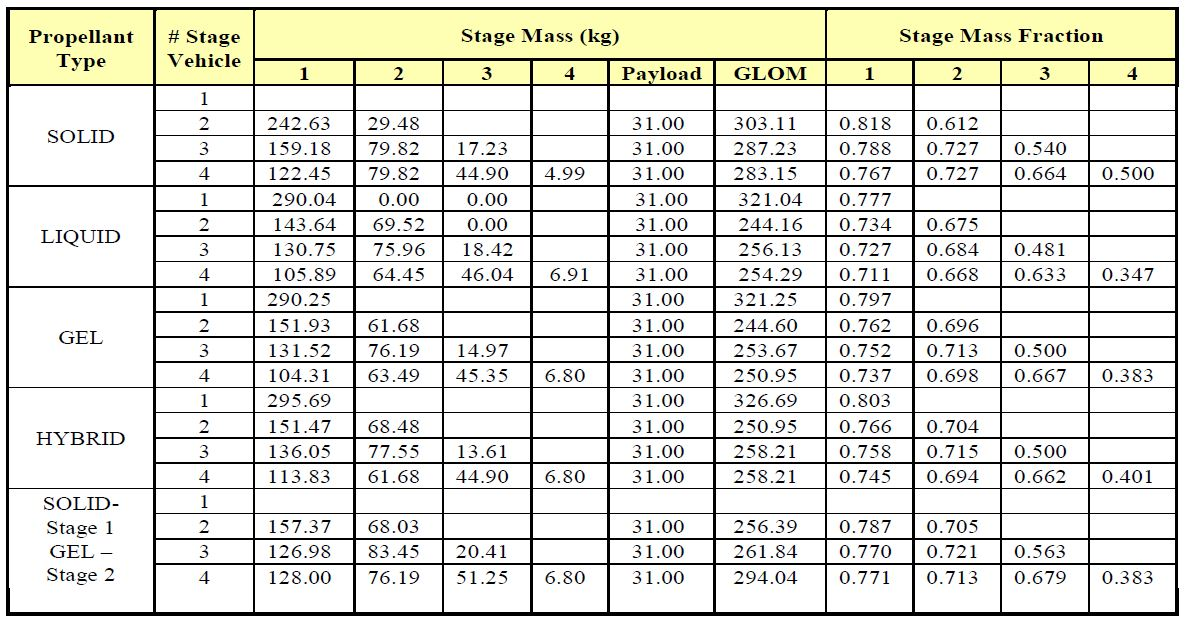
\includegraphics[width=0.9\textwidth]{figures/launcher_methods/examplestaging_trinidad2012.jpg}
%\caption{Image of comparison table for different stages with different propellants\cite{trinidad2012}}
%\label{fig:examplestaging_trinidad2012}
%\end{figure}

In \cite{trinidad2012} it is shown that the \ac{GLOM} would be lowest when using a two-stage liquid rocket. Nevertheless, a two-stage gel rocket would be a reasonable alternative. However, a low \ac{GLOM} is not the only requirement. A visual representation of some of the described designs is presented in \Cref{fig:diff_mav_trinidad2012_stephenson2002_mungas2012}.


\begin{figure}[!ht]
\centering
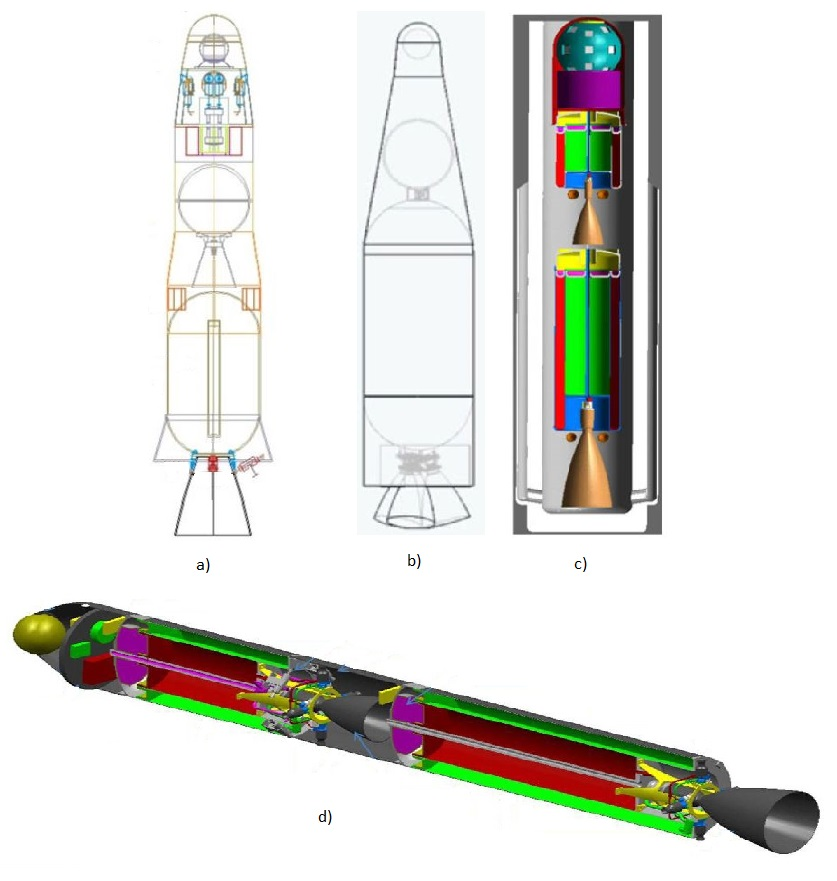
\includegraphics[width=0.7\textwidth]{figures/launcher_methods/diff_mav_trinidad2012_stephenson2002_mungas2012.jpg}
\caption{A number of rocket concepts visualized. a) Two-stage solid rocket by Lockheed Martin \cite{stephenson2002}, b) Single stage mono-liquid rocket by Firestar Technologies \cite{mungas2012}, c) Two-stage gel rocket by \ac{TRW} \cite{stephenson2002} and d) Two-stage bi-liquid rocket by Boeing and Northrop Grumman \cite{trinidad2012}.}
\label{fig:diff_mav_trinidad2012_stephenson2002_mungas2012}
\end{figure}

\subsection{Current \ac{MAV} baseline design}
\label{subsec:cur_mav_bas}
The latest baseline design for the \ac{MAV} originates from a (number of) studie(s) conducted in 2012 (also see \Cref{tab:refmavstud}). The main properties of the current baseline are presented best by \cite{trinidad2012}. In this paper, the rocket depicted in \Cref{fig:diff_mav_trinidad2012_stephenson2002_mungas2012},d) was analysed and put forward as the baseline design with the orbital sample container located in (and acting as) the nose of the rocket. A more detailed view of the baseline \ac{MAV} is shown in \Cref{fig:baseline_mav_trinidad2012}. Here, the samples are contained in the \ac{OS}, the thrust vector is controlled by the \ac{TVC} engines (or \ac{RCS}) and the final attitude adjustments are made by the \ac{ACS} thrusters.

\begin{figure}[!ht]
\centering
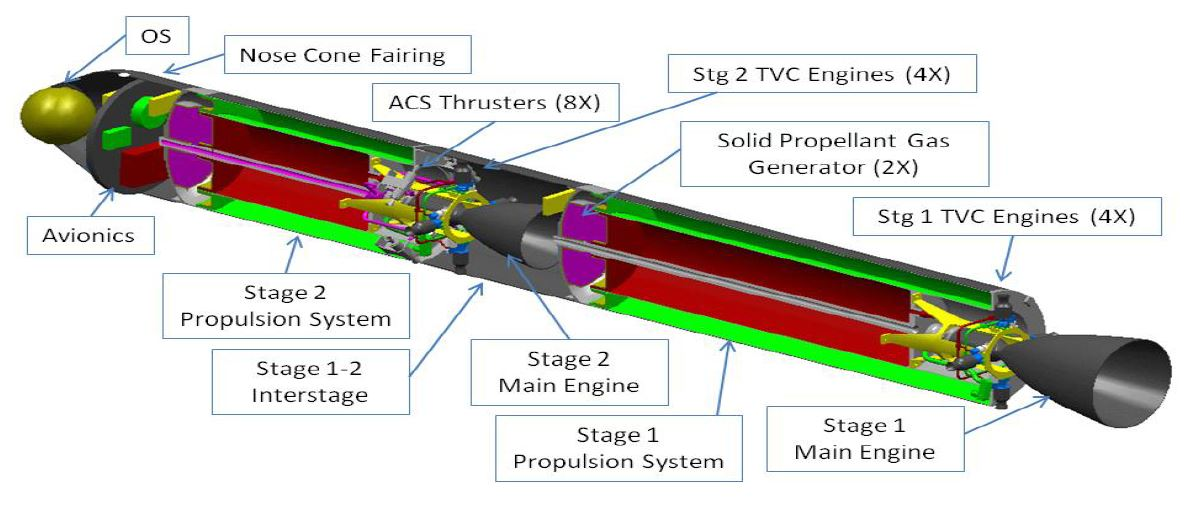
\includegraphics[width=0.7\textwidth]{figures/heritage/baseline_mav_trinidad2012.jpg}
\caption{Two-stage bi-liquid baseline \ac{MAV} with descriptions of different components \cite{trinidad2012}.}
\label{fig:baseline_mav_trinidad2012}
\end{figure}



The design resulted from the requirements for an \ac{MAV} put forward back in 2010. The main characteristics of the baseline \ac{MAV} are summarised in \Cref{tab:main_mav_bas_char}. It should be noted that since the current baseline design is a pressure-regulated system, the thrust is constant throughout the flight \cite{colozza2003comparison}.

%\textbf{\textcolor{red}{Need actual paper!!}}

\begin{table}[!ht]
\begin{center}
\caption{\ac{MAV} baseline design characteristics \cite{trinidad2012}.}
\label{tab:main_mav_bas_char}
\begin{tabular}{|l|l|}
\hline 
\textbf{Characteristic} 		&\textbf{Value or property}  \\ \hline \hline
Martian Sample Payload   &  5 kg  \\ \hline
Stage 1 main engine thrust   & 5.3 kN (restartable)   \\ \hline
Stage 2 main engine thrust   & 2.7 kN (restartable)  \\ \hline
Stage 1 \ac{RCS} engines   & 445 N (4x)    \\ \hline
Stage 2 \ac{RCS} engines   & 445 N (4x)    \\ \hline
Stage 2 \ac{ACS} engines   & 4.4 N (8x)  \\ \hline
Main engine propellants   & MON-25 (Oxidizer), MMH (Fuel) (2x)  \\ \hline
\ac{RCS} propellant (hot-gas)  &  Segmented solid propellant gas generators (also, liquid tank pressurant) \\ \hline
Total \ac{MAV} mass   & 227 kg (283 kg with contingencies and 391 kg with extreme contingencies)   \\ \hline
$I_{sp}$   &  330.5 s vacuum, 328.6 s in Martian atmosphere \\ \hline
Diameter   & 340 mm   \\ \hline
Total length   & approx. $\le$ 3666 mm \\ \hline
Max. launch angle   &  $\pm$ 35$^{\circ}$ off vertical axis  \\ \hline
Target orbit   & 460 by 580 km  \\ \hline
 		
% 		&   \\ \hline
\end{tabular}
\end{center}
\end{table} 

%In this baseline study, five different launch angles were studied and compared: 125, 95, 90, 85 and 55$^{\circ}$. Each of these launch angles had to result in the same trajectory after launch. Which is why directly after launch a coasting period was introduced (which is why the restart is important). During this coast phase the \ac{RCS} would be used to direct the main thrust into the near-optimal direction of the desired trajectory, after which the engine is re-ignited and continues on the set path. This is visualized in \Cref{fig:initial_coast_trinidad2012} in a vertical- vs. down-range plot.
%
%\begin{figure}[!ht]
%\centering
%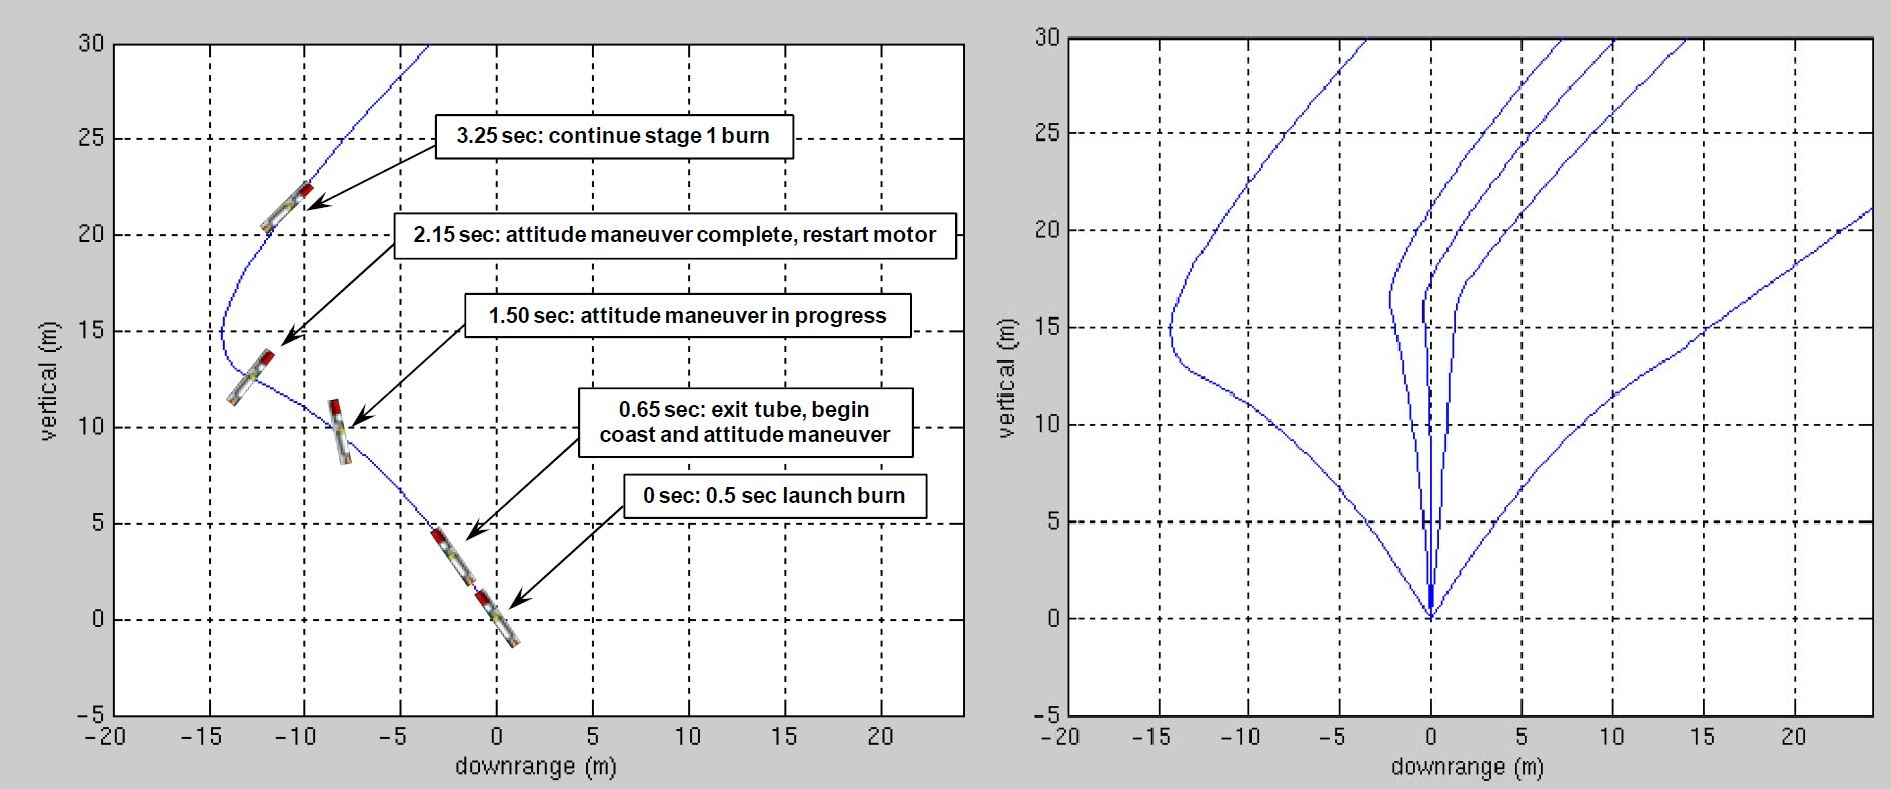
\includegraphics[width=1.0\textwidth]{figures/heritage/initial_coast_trinidad2012.jpg}
%\caption{Left: Initial trajectory and orientation of the \ac{MAV} for 125$^{\circ}$. Right: Comparison of the five analysed angles. \cite{trinidad2012}}
%\label{fig:initial_coast_trinidad2012}
%\end{figure}



\subsection{Current design restrictions}
\label{subsec:cur_des_rest}
The baseline design described in \Cref{subsec:cur_mav_bas} was based on early design restrictions set by the \ac{MAV} Study Guidelines 2010 (as mentioned in \cite{trinidad2012}). These include those specified in  \cite{anderson2011propulsion}. The restrictions provide flexibility in the design space (the upper and lower bound of the values specified in \Cref{tab:main_mav_bas_char}), should any of the baseline design parameters be changed slightly to result in a more optimum ascent. In this case, some design parameters could be treated as optimisation parameters (if required).
%  The design restrictions mentioned in \cite{trinidad2012} form the design space available for optimisation.

%  \textbf{\textcolor{red}{Need actual paper!!}}

\begin{itemize}
\item The total system, which is the \ac{MAV} and the erector support system (tower) to launch it, have to have a total mass of less than 360 kg \cite{trinidad2012}
\item Updated volume requirement: ranging from 3666 mm long with a diameter of 350 mm to 3150 mm long with a diameter of 700 mm \cite{trinidad2012}
\item 45$^{\circ}$ $\pm$ 0.2$^{\circ}$ target orbit inclination \cite{anderson2011propulsion}
\item Ability to launch from $\pm$ 30$^{\circ}$ latitudes \cite{anderson2011propulsion}
\item Sample sphere diameter: 16 cm (5 kg) \cite{anderson2011propulsion}
\end{itemize}
 





